
\documentclass{article} % For LaTeX2e
\usepackage{iclr2024_conference, times}

% Optional math commands from https://github.com/goodfeli/dlbook_notation.
%\input{math_commands.tex}

\usepackage{hyperref}
\usepackage{url}


%%%%%%%%%%%%%%%%%%%%%%%%%%%%%%%%%%%%%%%%%%%%%%%%%%%%%%%%%%%%%%%%%%%%%%%%%%%%%%%%%%%%%%%%%%%%
\usepackage{amsthm,mathtools,amsfonts,amssymb, color, relsize, enumerate, enumitem}
\usepackage{relsize}
\usepackage{subfloat}
\usepackage{algorithm}
\usepackage{algpseudocode}

\usepackage{float}

\usepackage{geometry}
\usepackage{setspace}

\newtheoremstyle{bfnote}%
{}{}
{\itshape}{}
{\bfseries}{.}
{ }{\thmname{#1}\thmnumber{ #2}\thmnote{ (#3)}}
\theoremstyle{bfnote}

\newtheorem{theorem}{Theorem}[section]
\newtheorem{lemma}[theorem]{Lemma}
\newtheorem{proposition}[theorem]{Proposition}
\newtheorem{definition}[theorem]{Definition}
\newtheorem{corollary}[theorem]{Corollary}
\newtheorem{remark}[theorem]{Remark}
\newtheorem{assumption}[theorem]{Assumption}
\newtheorem{claim}[theorem]{Claim}
\newtheorem{observation}[theorem]{Observation}

\usepackage{listings}
\usepackage{appendix}
\usepackage{wrapfig}
\usepackage{rotating}
\usepackage{subfig}

\usepackage{booktabs}
\usepackage{colortbl}

\usepackage[c]{esvect}

% To get a bold Greek letter.
\usepackage{bm}

\usepackage{xcolor}

\usepackage{pdfpages}

\usepackage{multirow}
\usepackage{booktabs}

\usepackage[nameinlink, capitalise, noabbrev]{cleveref}
\crefname{section}{Sec.}{Secs.}
\Crefname{equation}{Eq.}{Eqs.}
\Crefname{figure}{Fig.}{Figs.}
\Crefname{tabular}{Tab.}{Tabs.}
\Crefname{table}{Tab.}{Tabs.}
\crefname{listing}{Algorithm.}{Algorithms.}
\crefname{appendix}{App.}{Apps.}
\creflabelformat{equation}{#2\textup{#1}#3}  % <- remove parenthesis from equations

\definecolor{rasbery}{HTML}{b00149}
\definecolor{redpink}{HTML}{fe2c54}
\definecolor{neonblue}{HTML}{c6fcff}
\definecolor{oceanblue}{HTML}{03719c}
\definecolor{brickred}{HTML}{8f1402}
\definecolor{skyblue}{HTML}{75bbfd}
\definecolor{yelloworange}{HTML}{fcb001}
\definecolor{oliviegreen}{HTML}{4b5d16}
\definecolor{lightpink}{HTML}{ffd1df}
\definecolor{lightpurple}{HTML}{eecffe}
\definecolor{lightsalmon}{HTML}{fea993}
\definecolor{neonyellow}{HTML}{cfff04}

\usepackage[colorinlistoftodos, prependcaption, textsize=tiny, tickmarkheight=12]{todonotes}
\newcommand{\addref}[2]{\todo[inline, inlinewidth=5cm, color=lightpink, author=#2]{#1}}
\newcommand{\addtable}[2]{\todo[inline, inlinewidth=5cm, color=lightsalmon, author=#2]{#1}}
\newcommand{\adddetail}[2]{\todo[inline, inlinewidth=5cm, author=#2, color=lightpurple]{#1}}
\newcommand{\addfigure}[2]{\missingfigure[inline, inlinewidth=5cm, figwidth=#1, figcolor=yelloworange]{#2}}
\newcommand{\moveit}[2]{\todo[inline, inlinewidth=5cm, author=#2, color=neonyellow]{#1}}
\newcommand{\dcheck}[2]{\todo[inline, inlinewidth=5cm, author=#2, color=neonblue]{#1}}
% # CODE SNIPPETS

\definecolor{strings}{rgb}{.624,.251,.259}
\definecolor{keywords}{rgb}{.224,.451,.686}
\definecolor{comment}{rgb}{.322,.451,.322}

\usepackage{minted}
\newminted{python}{fontsize=\footnotesize, mathescape=true, escapeinside=@@}

\usepackage{tikz, pgf}
\usetikzlibrary{arrows,shapes, decorations.pathmorphing,backgrounds,positioning}
\pgfdeclarelayer{background}
\pgfsetlayers{background,main}


% https://tinyurl.com/ysaxzhbd
\expandafter\def\expandafter\normalsize\expandafter{%
	\normalsize%
	\setlength\abovedisplayskip{4pt}%
	\setlength\belowdisplayskip{8pt}%
	\setlength\abovedisplayshortskip{2pt}%
	\setlength\belowdisplayshortskip{5pt}%
}

%\setlength{\parskip}{0.25cm}
%%%%%%%%%%%%%%%%%%%%%%%%%%%%%%%%%%%%%%%%%%%%%%%%%%%%%%%%%%%%%%%%%%%%%%%%%%%%%%%%%%%%%%%%%%%%%%%%

\title{Formatting Instructions for ICLR 2024 \\ Conference Submissions}

% Authors must not appear in the submitted version. They should be hidden
% as long as the \iclrfinalcopy macro remains commented out below.
% Non-anonymous submissions will be rejected without review.

\author{Antiquus S.~Hippocampus, Natalia Cerebro \& Amelie P. Amygdale \thanks{ Use footnote for providing further information
		about author (webpage, alternative address)---\emph{not} for acknowledging
		funding agencies.  Funding acknowledgements go at the end of the paper.} \\
	Department of Computer Science\\
	Cranberry-Lemon University\\
	Pittsburgh, PA 15213, USA \\
	\texttt{\{hippo,brain,jen\}@cs.cranberry-lemon.edu} \\
	\And
	Ji Q. Ren \& Yevgeny LeNet \\
	Department of Computational Neuroscience \\
	University of the Witwatersrand \\
	Joburg, South Africa \\
	\texttt{\{robot,net\}@wits.ac.za} \\
	\AND
	Coauthor \\
	Affiliation \\
	Address \\
	\texttt{email}
}

% The \author macro works with any number of authors. There are two commands
% used to separate the names and addresses of multiple authors: \And and \AND.
%
% Using \And between authors leaves it to \LaTeX{} to determine where to break
% the lines. Using \AND forces a linebreak at that point. So, if \LaTeX{}
% puts 3 of 4 authors names on the first line, and the last on the second
% line, try using \AND instead of \And before the third author name.

\newcommand{\fix}{\marginpar{FIX}}
\newcommand{\new}{\marginpar{NEW}}
%%%%%%%%%%%%%%%%%%%%%%%%%%%%%%%%%%%%%%%%%%%%%%%%%%%%%%%%%%%%%%%%%%%%%%%%%%%%%%%%%%%%%%%%%%%%%
%\iclrfinalcopy % Uncomment for camera-ready version, but NOT for submission.

\begin{document}

	
\title{Unifying Feature Attribution: Bridging Attention Mechanisms and Shapley Values}
\maketitle

\begin{abstract}
	Machine learning (ML) applications have become ubiquitous in various domains, including  and large language models and computer vision. However, the increasing prevalence of ML models has also emphasized the need for explainable artificial intelligence (XAI). In particular, it has become crucial to develop techniques that can help explain how these models work and why they make certain decisions. This is especially important in cases where these models are used to make critical decisions that can have significant consequences on individuals or society as a whole.
\end{abstract}

\section{Introduction}
%Machine learning (ML) applications have become ubiquitous in various domains, including  and large language models and computer vision. However, the increasing prevalence of ML models has also emphasized the need for explainable artificial intelligence (XAI). In particular, it has become crucial to develop techniques that can help explain how these models work and why they make certain decisions. This is especially important in cases where these models are used to make critical decisions that can have significant consequences on individuals or society as a whole.
%
%Three primary methods for evaluating feature attribution in machine learning models are Shapley values, gradient-based, and perturbation-based methods. Although these methods aim to reveal the contribution of individual features to model predictions, they differ in their underlying principles and techniques.
%
%\begin{itemize}
%	\item \textbf{Perturbation-based methods}: these methods are a way of determining the significance of input features in a neural network. This is done by modifying the values of certain features and observing the effect of these changes on the network's performance. However, this approach is quite computationally intensive because it requires multiple passes through the network to assess the importance of each input pixel. Consequently, perturbation-based attribution methods can be quite time-consuming.
%	
%	\item \textbf{Gradient-based methods}: these methods work by analyzing the gradients of the model's output in relation to input features. This involves calculating the gradients of the output (logits or soft-max probabilities) with respect to the extracted features or input, using backpropagation. These gradients are then utilized to estimate attribution scores. However, the gradients tend to be noisy, which may result in attribution maps that show contributions from irrelevant features.
%	
%	\item \textbf{Shapley values}: Shapley values, a concept rooted in cooperative game theory, offers a comprehensive and theoretically grounded approach to distribute the contribution of each feature fairly across different predictions. Essentially, the framework considers all possible feature combinations and evaluates the marginal contribution of each feature within these combinations. This way, each feature receives an unbiased and fair attribution based on its contribution to the overall prediction.
%	
%	\smallskip
%	Shapley values can be very difficult to compute, particularly when there are a large number of contributors or features involved. This is because calculating them requires considering all possible permutations of contributors in a cooperative game, which lead to exponential computations. Researchers often use approximations or sampling techniques, but applying Shapley values to high-dimensional and real-world machine learning problems remains a significant challenge.
%\end{itemize}
%
%
%The integration of attention mechanisms in machine learning has improved the accuracy of models and offered a solution to the interpretability issue faced by complex models in natural language processing. Attention weights are crucial in understanding NLP tasks, revealing a meaningful connection between a word's attention weight and its contribution to the final predictions. This connection suggests a monotonic relationship, where higher assigned weights indicate greater importance of the corresponding word in NLP tasks.
%
%It is worth noting that attention-based explanations present their own set of challenges. One of the challenges is that each feature calculates attention to other layers' features, creating a continuous cycle during backpropagation iterations. As a result, it becomes difficult to precisely interpret attention as an explanation since it is heavily influenced by other features' embeddings after just a few iterations. Additionally, the significance of initial attention weights may be less informative since randomized initialization has a significant impact. Even when these aspects are considered, there is still considerable controversy surrounding the interpretation of attention mechanisms.

In the pursuit of transparent and interpretable machine learning models, understanding feature attribution methods is pivotal. Feature attribution elucidates the contribution of individual input elements to model predictions, fostering model interpretability. However, existing methods grapple with challenges, such as non-uniqueness and interpretability gaps. In this paper, we present a cohesive framework by leveraging attention mechanisms and Shapley values. 

The attention mechanism, initially designed for natural language processing, has proven instrumental in capturing contextual relationships within input data. Simultaneously, Shapley values, rooted in cooperative game theory, provide a principled approach to distributing contributions among features. We propose a novel integration of attention and Shapley values, unifying their strengths to yield robust and interpretable feature attributions.

\textbf{Contribution}:\\ 
Our approach addresses the challenges faced by existing methods, offering a more nuanced understanding of feature importance. Through empirical evaluations on diverse datasets, we demonstrate the effectiveness and versatility of our proposed method in enhancing interpretability across various machine learning models.

\dcheck{Quality of Writing}{Max}
\adddetail{Our Contributions?}{Behrooz+Max}

%The assertion that both Shapley and attention values are deemed 'interpretable' raises a compelling question in the domain of XAI. It prompts a nuanced exploration of these two interpretability frameworks' similarities and potential equivalence.


\section{Related Works}
The concept of attention flows was introduced by \cite{abnar2020b} and presented a new perspective on how XAI could leverage attention flows. However, the authors of the paper chose to focus on simple ideas that only required attention weights, which could be easily implemented in any architecture employing self-attention mechanism. While they compared attention flows with other concepts like attention rollout, they did not employ maximum flow to obtain the attribution of each token in language models. In the classification task, they conducted an evaluation of the weights obtained from raw attention, attention rollout, and attention flow for the CLS embedding over input tokens in all attention layers for a selected set of examples. In the masked language modeling task, a similar analysis was performed on the quantities derived from the MASK embedding to the two potential references.

In a recent study, \cite{ethayarajh2021b} attempted to establish a systematic connection between attention flows and XAI. While their work focused on demonstrating that attention flows can be interpreted as Shapley values under certain conditions, they did not account for the non-uniqueness of such flows. It is worth noting that, although maximum flow problem has the unique optimal value, there can be multiple feasible flows that attain this optimal value. 

This highlights the need for further research to explore the method to resolve the issue of non-uniqueness in attention flows and its impact on XAI.

\section{Preliminaries}
We will define preliminary terms and definitions here that will be used in the subsequent sections. This study will primarily utilize these concepts.

\subsection{Graph Network Flow}

\subsubsection{Maximum Flow}
\begin{definition}[Network Flow]
	Given a network $G=(V, E, s, t, \bm{u})$, where $s$ and $t$ are the source and target nodes respectively and $u_{i j}$ is the capacity for the edge $(i,j)\in E$, a flow is characterized as a function \( f: E \rightarrow \mathbb{R}^{\geq 0} \) s.t.
	
	\begin{equation}
		\arraycolsep=3pt
		\def\arraystretch{1.5}
		\begin{array}{ll}
			f_{i j} \leq u_{i j} \quad \forall(i, j) \in E \hspace{8pt} \text{(capacity constraints)} \\
			\vspace{4pt}
			\mathlarger{\mathlarger{\sum\limits_{j:(i, j) \in E}}} f_{i j} - \hspace{-3pt} \mathlarger{\mathlarger{\sum\limits_{j:(j, i) \in E}}} f_{j i} = 0, \quad \forall i \in V, i \neq s, t \hspace{8pt} \text{(flow conservation constraints)}
		\end{array}
		\label{eq:1}
	\end{equation}
\end{definition}
	
The value of a flow in a given network \( G = (V, E, s, t, \bm{u}) \) is established as the sum of flows into the source vertex \( s \), denoted as \( |f| = \sum_{v:(s, v)} f_{s v} \), and a maximum flow is identified as a feasible flow with the highest attainable value. We define $\left|f_{out}(i)\right|$ to be the total outflow value of a node $i$ and $\left|f_{in}(i)\right|$ to be the total inflow value of a node $i$. For a given set $K \subseteq V$ of nodes, we define $|f(K)|= \sum_{i \in K}|f_{out}(i)|$ for every flow $f$.

 \adddetail{Check definition of val(f)}{Behrooz}



\subsubsection{Minimum-Cost Circulation}
\begin{definition}[Minimum Cost Circulation]
	Given a network $G=(V, E, \bm{u}, \bm{l}, \bm{c})$ with $ |V|=n $ vertices and $ |E|=m $ edges, where $c_{i j}$ is the cost, $l_{i, j}$ and $u_{i, j}$ are respectively the lower and upper capacities for the edge $(i,j)\in E$, a circulation is f function $f: E \rightarrow \mathbb{R}^{\geq 0}$ s.t.
	
	\begin{equation}
		\arraycolsep=3pt
		\def\arraystretch{1.5}
		\begin{array}{ll}
			l_{i j} \leq f_{i j} \leq u_{i j}, & \forall(i, j) \in E \\
			\mathlarger{\mathlarger{\sum\limits_{j:(i, j) \in E}}} f_{i j} - \hspace{-3pt} \mathlarger{\mathlarger{\sum\limits_{j:(j, i) \in E}}} f_{j i} = 0, & \forall i \in V .
		\end{array}
		\label{eq:3}
	\end{equation}
	
	The min-cost circulation problem is to find a circulation $f$ that minimizes the cost function $\mathlarger{\sum_{(i, j) \in E}} c_{i j} f_{i j}$. 
	
\end{definition}


The formulation of minimum-cost circulation problem can be algebraically written as the following linear programming (LP) problem:
\begin{equation}
	\underset{\substack{\bm{B}^{\top} \bm{f}=\bm{0} \\ l_e \leq f_e \leq u_e \forall e \in E}}{\min } \hspace{-4pt} \bm{c}^{\top} \bm{f} \quad  \text{i.e.}	\quad 
	\underset{\substack{\bm{B}^{\top} \bm{f}=\bm{0} \\ \bm{l} \leq \bm{f} \leq \bm{u} }}{\arg \min } \hspace{4pt} \bm{c}^{\top} \bm{f}	
	\label{eq:5}
\end{equation}

where $B_{m \times n}$,is the edge-vertex incidence matrix.
For a directed graph, the entries of the matrix $ \bm{B} $ are defined as follows:
\vspace{-2pt}
\begin{equation*}
	b_{e v} =
	\begin{cases}
		-1, & \text{if vertex } v \text{ is the tail of edge } e, \\
		1,  & \text{if vertex } v \text{ is the head of edge } e, \\
		0,  & \text{if edge } v \text{ is not incident to vertex } e.
	\end{cases}
\end{equation*}

\subsection{Shapley Values}
\begin{definition} [Shapley Values]
	Shapley values are defined through value functions $\vartheta$ of subsets $S$ of players in a set $N=$ $\{1,2, \ldots, n\}$. Specifically, the Shapley value $\phi_i(\vartheta)$ of player (or feature) $i$ in a game with total payoff $v$ is given by:
\end{definition}

\begin{equation}
	\phi_i(\vartheta)=\mathlarger{\sum\limits_{S \subseteq N \backslash\{i\}}} \frac{|S| !(n-|S|-1) !}{n !}(\vartheta(S \cup\{i\})-\vartheta(S))
	\label{eq:4}
\end{equation}

\begin{remark}
Shapley values are the unique linear additive explanation that satisfies four fairness-based axioms (efficiency, symmetry, linearity (additivity), and null player)
\end{remark} Please see Appendix A for details.

\subsection{Multi-Head Attention Mechanism}
Given an input sequence $\bm{X}\in \mathbb{R}^{t \times d}$, where $d$ is the dimensionality of the model's input vectors, the multi-head self-attention mechanism computes attention weights for each element in the sequence.

\begin{itemize}
	\item \textbf{Linear Transformation}:
	\[
	\bm{Q}_i = \bm{XW}^Q_{i}, \quad \bm{K}_i = \bm{XW}^K_{i}, \quad \bm{V}_i = \bm{XW}^V_{i}
	\]
	where \(\bm{Q}_i, \bm{K}_i, \bm{V}_i \in \mathbb{R}^{t \times d_k}\), and \(\bm{W}^Q_{i}, \bm{W}^K_{i}, \bm{W}^V_{i} \in \mathbb{R}^{d \times d_k}\).
	
	\item \textbf{Scaled Dot-Product Attention}:
	\[
	\text{Attention}_{i}(\bm{Q}_i, \bm{K}_i, \bm{V}_i) = \text{softmax}\left(\frac{\bm{Q}_i\bm{K}_i^T}{\sqrt{d_k}}\right) \bm{V}_i
	\]
	
	where the division by \(\sqrt{d_k}\) is for scaling. Here \( \text{Attention}_{i}\) represent the operation for the \(i\)-th head, and the attention scores matrix $\widetilde{\bm{A}}_i$ for the $i$-th head is defined as:
	
	\begin{equation}
		\widetilde{\bm{A}}_i = \text{softmax}\left(\frac{\bm{Q}_i\bm{K}_i^T}{\sqrt{d_k}}\right)
	\end{equation}

	
	Here, $n$ is the sequence length, $d$ is the dimensionality of the model's input vectors, and $d_k$ is the dimensionality of the key vectors. The resulting matrix $\widetilde{\bm{A}}_i$ has dimensions $\widetilde{\bm{A}}_i \in \mathbb{R}^{t \times t}$, where each element $\widetilde{\bm{A}}_i(j, k)$ represents the attention weight assigned to the $j$-th element when processing the $k$-th element in the sequence. 
	
	
	\item \textbf{Concatenation and Linear Projection}:
	
	\[
	\text{MultiHead}(\bm{X}) = \text{Concat}(\text{Attention}_1, \text{Attention}_2, \ldots, \text{Attention}_h)\bm{W}_O
	\]
	
	where \(\text{MultiHead}(\bm{X}) \in \mathbb{R}^{t \times d}\), and \(\bm{W}_O \in \mathbb{R}^{h \cdot d_k \times d}\).
	
	For a transformer architecture with $l$ attention layers, the attention scores at each layer can be defined as multi-head attention score:
	 \begin{equation}
	 \bm{\widehat{A}} = \text{Concat}(\widetilde{\bm{A}}_1, \widetilde{\bm{A}}_2, \cdots, \widetilde{\bm{A}}_h) \in \mathbb{R}^{h \times t \times t}
	 \end{equation}
	 
	 We can extend this concept to a transformer architectures itself as following:
	 \begin{equation}
	 		 \bm{A}=\text{Concat}(\bm{\widehat{A}}_1, \bm{\widehat{A}}_2, \cdots, \bm{\widehat{A}}_l) \in \mathbb{R}^{l \times h \times t \times t}
	 \end{equation}
	wehre $\widehat{A}_j \in \mathbb{R}^{h \times t \times t}$ is the multi-head attention score for $j$-th attention layer.
\end{itemize}


\section{Methods}

\subsection{Non-uniqueness of Maximum Flow}
%\begin{definition}[Residual Graph]
%	The residual graph for a circulation $f$ is $G_f=\left(V, E_f\right)$ where $E_f=\{(i, j) \in$ $\left.E: l_{i j} \leq f_{i j} \leq u_{i j}\right \}$ with the new capacity constraints  $u^f_{i j}=u_{i j}-f_{i j}$ and  $l^f_{i j}=l_{i j}-f_{i j}$ and the same cost $c_{i j}$.
%\end{definition}
%
%
%\begin{theorem}[Optimality of Circulation]\citep{kargera}
%	A circulation is optimal (min-cost) if and only if the corresponding residual graph $G_f$ does not have a feasible circulation of negative cost.
%	\label{theorem:1}
%\end{theorem}
%
%Employing \cref{theorem:1} enables us to easily determine whether the minimum cost circulation problem has a unique optimal circulation within a polynomial time complexity. 

It should be noted that the problem at hand is not strictly convex, which implies that the existence of a unique solution cannot be guaranteed. Additionally, we have discovered that the maximum flow problem for the previously constructed graph does not possess a unique solution either. Specifically, we have identified two feasible maximum flows for a similar graph created using attention flows. These maximum flows can be obtained using two distinct algorithms, namely \cref{algo:1} and \cref{algo:2}.


Moreover, we know that if any linear programming has two distinct feasible solutions $f_1$, $f_2$, any convex combination $\gamma_1 f_1 + \gamma_2 f_2$ where $\gamma_1+\gamma_2=1$ is a new solution. Consequently, the attention flows has infinite feasible solution and therefore the feature attributions and Shapley values resulted from this approach is ill-defined.  


%\begin{observation}[Polynomial-Time Algorithm for Uniqueness of Maximum Flow]
%To ascertain whether the feasible circulation for the minimum cost circulation problem is unique or not, one can create a residual network and employ Depth First Search (DFS) on the graph. If DFS reveals a cycle in the residual graph, it indicates that there exists another maximum flow solution where the flow on at least one edge is distinct.
%\end{observation}

\subsection{Make Maximum Flow Unique}
As previously discussed, each network inherently possesses a distinct maximum flow value. However, achieving this maximum value is not confined to a singular feasible flow; rather, multiple feasible flows can attain the same maximum. This variability introduces a challenge in discerning the optimal flow solution. To address this challenge, the introduction of regularization terms into the maximum flow problem proves beneficial. Through this regularization, the objective of the linear programming problem defined in \cref{eq:5} is transformed into a strictly convex function. This transformation ensures the derivation of a unique and optimal approximate solution, thereby overcoming the issue posed by the non-uniqueness of feasible flows achieving the maximum value.

Here we introduce two main regularization term and the logic behind them: 1. log-barrier regularization 2. $\ell _1$ and $\ell_2$ regularization.

\subsubsection{Log-Barrier Regularization}
We can reformulate the minimum cost circulation problem as:
\begin{equation}
	\underset{\substack{\bm{B}^{\top} \bm{f}=\bm{0} \\ h(\bm{f}) \leq \bm{0} }}{\arg \min } \hspace{4pt} \bm{c}^{\top} \bm{f}
	\label{eq:8}
\end{equation}
where $h(\bm{f}) = (\bm{f}-\bm{l}) (\bm{f}-\bm{u})$. 

Defining the log-barrier function $\phi_{\mu}(\bm{f})=-\mu \mathlarger{\sum\limits_{e \in E}} \log \left(-h(f_e)\right) = \mu \mathlarger{\sum\limits_{e \in E}} \left( \log \left(f_e-l_e\right) +\log \left(u_e-f_e\right) \right)$, the original problem can, therefor, be approximated using the log barrier function as the following:
\begin{equation}
	\begin{array}{ll}
		\underset{\substack{\bm{B}^{\top} \bm{f}=\bm{0}}}{\arg \min } \hspace{2pt} \bm{c}^{\top} \bm{f} + \Phi_{\mu}(\bm{f}) %= & \\
%		\underset{\substack{\bm{B}^{\top} \bm{f}=\bm{0}}}{\arg \min } \hspace{2pt} \bm{c}^{\top} \bm{f} + \mu \mathlarger{\sum\limits_{e \in E}} \left( \log \left(f_e-l_e\right) +\log \left(u_e-f_e\right) \right)
	\end{array}
	\label{eq:9}
\end{equation}


%which is equivalent to
%\begin{equation}
%	\begin{array}{rl}
	%		\underset{\substack{\bm{B}^{\top} \bm{f}=\bm{0}}}{\arg \min } \hspace{2pt} \bm{c}^{\top} \bm{f} +\mathbb{I}_C(\bm{f}) \\
	%	\end{array}
%\end{equation}
%
%where $h(f_e) = (f_e-l_e) (f_e-u_e) \hspace{2pt}$ for any edge $e$ and the feasible set $C$ is defined as:
%\begin{equation}
%	C:=\left\{ \bm{f}: h(\bm{f}) \leq \bm{0}\right\} = \left\{f: h(f_e) \leq 0, \forall e \in E \right\}
%\end{equation}


It is easy to observe that as long as $\mu>0$ and our initial solution is feasible, the barrier function will ensure that any solution we find using an iterative minimization scheme, such as gradient descent or Newton's method, remains feasible. Moreover, one can show that to get an $\varepsilon$-approximate solution to the \cref{eq:8} it suffices to set $\mu \leq \frac{\varepsilon}{2 m}$ and find the optimal solution to the corresponding problem in \cref{eq:9}.\citep{boyd2004, bubeck2015}

Finally, observe that the Hessian of the objective function of \cref{eq:9} at some point $\bm{f}$ is equal to the Hessian $\nabla^2 \Phi_\mu(x)$ of the barrier function. The latter turns out to be a diagonal matrix with
\begin{equation*}
	\left(\nabla^2 \Phi_\mu(\bm{f})\right)_{e, e}=\mu\left(\frac{1}{\left(u_e-f_e\right)^2}+\frac{1}{\left(f_e-l_e\right)^2}\right),
\end{equation*}
for each edge $e$. Thus, the Hessian of our objective function is positive definite (provided $\mu>0)$, which implies that the objective function is strongly convex and therefore have a unique feasible solution.

There are many preceding study about various numerical methods and their convergence rate which we leave the readers for further investigation \citep{bertsimas1997, boyd2004, bubeck2015}. It is noteworthy to mention that many other barrier functions can be used instead of log-barrier functions which can enhance the convergence rate of numerical solver for the optimization problem. \citep{cohen2020, lee2020, axiotis2022, brand2021c, chen2022a}

\subsubsection{$\ell_1 \hspace{2pt }\text{and}  \hspace{2pt}  \ell_2$ Regularization}

L1 regularization encourages sparsity in the model, which means it forces some of the feature weights to be precisely zero. This leads to feature selection, where only a subset of the most relevant features is retained in the model, which is particularly useful when dealing with high-dimensional datasets or when there is a suspicion that many features may not contribute significantly to the model's performance. On the other hand, L2 regularization constrains the magnitude of the weights, preventing them from becoming too large. L2 regularization ensures a more stable and generalized model by penalizing overly complex models with large coefficients \citep{yena}.

Therefore, we can regularize the \cref{eq:8} as:
\begin{equation}
	\underset{\substack{\bm{B}^{\top} \bm{f}=\bm{0} \\ h(\bm{f}) \leq \bm{0} }}{\arg \min } \hspace{4pt} \bm{c}^{\top} \bm{f} +\lambda_1 \|\bm{f}\|_1 +\lambda_2 \|\bm{f}\|_2^2
	\label{eq:10}
\end{equation}

where $\lambda_1, \lambda_2 >0$. It is is easy to show that to get an $\varepsilon$-approximate solution to the \cref{eq:8} it suffices to set $\max(\lambda_1, \lambda_2) \leq \frac{\varepsilon}{2} \min(1, \frac{1}{m \|\bm{u}\|_{\infty}})$ and find the optimal solution to the corresponding problem in \cref{eq:10}.\citep{boyd2004, bubeck2015}

\subsubsection{Attribution Flows}
One way to integrate the attention mechanism into XAI is by implementing a flow network representation of the graph. This representation assigns capacities to the edges of the graph that correspond to attention weights or similar values. By implementing a maximum flow algorithm, we can discover the flow from any node in any layer to any input node, which can help us estimate the quantity of attention (attribution) directed towards the input nodes.

To determine the maximum flow from all output nodes to all input nodes, we must utilize the concept of multi-commodity flow. This involves creating a super-source $s$ and a super-target $t$ with a capacity $u_{\infty}$. The connectivity between layers is established by means of attention weights or similar values, resulting in the formation of a layered network.

To formalize this process, assume we have the transformer architecture with $l$ attention layers , input sequence $X\in \mathbb{R}^{t \times d}$ and its attribution tensor $\bm{F} \in \mathbb{R}^{l \times t \times t}$. We create the multi-partite attribution graph $\mathcal{G}$ with its capacity matrix $\mathcal{F}$ and its integral version $\widetilde{\mathcal{F}}$ employing either \cref{algo:1} or \cref{algo:2}:

\begin{figure}[!htbp]
	\centering
	\begin{minipage}{0.45\textwidth}
		\begin{algorithm}[H]
			\footnotesize
			\begin{algorithmic}[0]
				\Require $\bm{F}_{l\times t \times t}$: An attribution tensor.
				\Ensure Tuple: $(\mathcal{F}, \widetilde{\mathcal{F}})$
				\Function{get\_attention\_flow}{$\bm{F}$}
				\State $l, t, \text{$\_$} \gets$ \text{$\bm{F}$.shape()}
				\State $\text{$\beta_{\min}$} \gets \min(\bm{F}>0)$
				\State $\text{$\beta$} \gets -\lfloor \log_{10}(\text{$\beta_{\min}$}) \rfloor$
				\State $\gamma \gets 10^\beta$
				\State $Q_{tl} \gets t \ast (l + 1) + 2$
				\State $\mathcal{\mathcal{F}} \gets \text{np.zeros} (Q_{tl}, Q_{tl})$
				\State $u_{\infty} \gets t$
				%	\Comment{Source and Sink: infinity capacity}
				\For{$i$ \text{ in range}($t$)}
				\State $\mathcal{F}[i+1][0] \gets u_{\infty}$
				\EndFor
				
				\For{$i$ \text{ in range}($t$)}
				\State $\mathcal{F}[-1][-i-2] \gets u_{\infty}$
				\EndFor
				\For{$j$ \text{ in range}$(0, l)$}
				\State $\text{low}, \text{up} \gets t \ast j + 1, t \ast (j + 1) + 1$
				\State $\mathcal{F}[\text{up} : \text{up}+t, \text{low} : \text{low}+t] \gets \bm{F}[j]$
				\EndFor
				\State $\widetilde{\mathcal{F}} \gets\text{int}(\gamma \ast \mathcal{F})$
				\EndFunction
			\end{algorithmic}
			\caption{Backward Attribution Flow}\label{algo:1}
		\end{algorithm}
	\end{minipage}
	\hfill
	\begin{minipage}{0.45\textwidth}
		\begin{algorithm}[H]
			\footnotesize
			\begin{algorithmic}[0]
				\Require $\bm{F}_{l\times t \times t}$: An attribution tensor.
				\Ensure Tuple: $(\mathcal{F}, \widetilde{\mathcal{F}})$
				\Function{get\_attention\_flow}{$\bm{F}$}
				\State $l, t, \text{$\_$} \gets$ \text{$\bm{F}$.shape()}
				\State $\text{$\beta_{\min}$} \gets \min(\bm{F}>0)$
				\State $\text{$\beta$} \gets -\lfloor \log_{10}(\text{$\beta_{\min}$}) \rfloor$
				\State $\gamma \gets 10^\beta$
				\State $Q_{tl} \gets t \ast (l + 1) + 2$
				\State $\mathcal{\mathcal{F}} \gets \text{np.zeros} (Q_{tl}, Q_{tl})$
				\State $u_{\infty} \gets t$
				%	\Comment{Source and Sink: infinity capacity}
				\For{$i$ \text{ in range}($t$)}
				\State $\mathcal{F}[i+1][0] \gets u_{\infty}$
				\EndFor
				
				\For{$i$ \text{ in range}($t$)}
				\State $\mathcal{F}[-1][-i-2] \gets u_{\infty}$
				\EndFor
				\For{$j$ \text{ in range}$(0, l)$}
				\State $\text{low}, \text{up} \gets t \ast j + 1, t \ast (j + 1) + 1$
				\State $\mathcal{F}[\text{up} : \text{up}+t, \text{low} : \text{low}+t] \gets \bm{F}[j]$
				\EndFor
				\State $\widetilde{\mathcal{F}} \gets\text{int}(\gamma \ast \mathcal{F})$
				\EndFunction
			\end{algorithmic}
			\caption{Forward Attribution Flow}\label{algo:2}
		\end{algorithm}
	\end{minipage}

\end{figure}
%\adddetail{check the algorithm accuracy add source and node indices to algorithms}{Behrooz}

%\begin{figure}[H]%
%	\hspace{-2cm}
%	\subfloat[backward attribution flow]{
%		{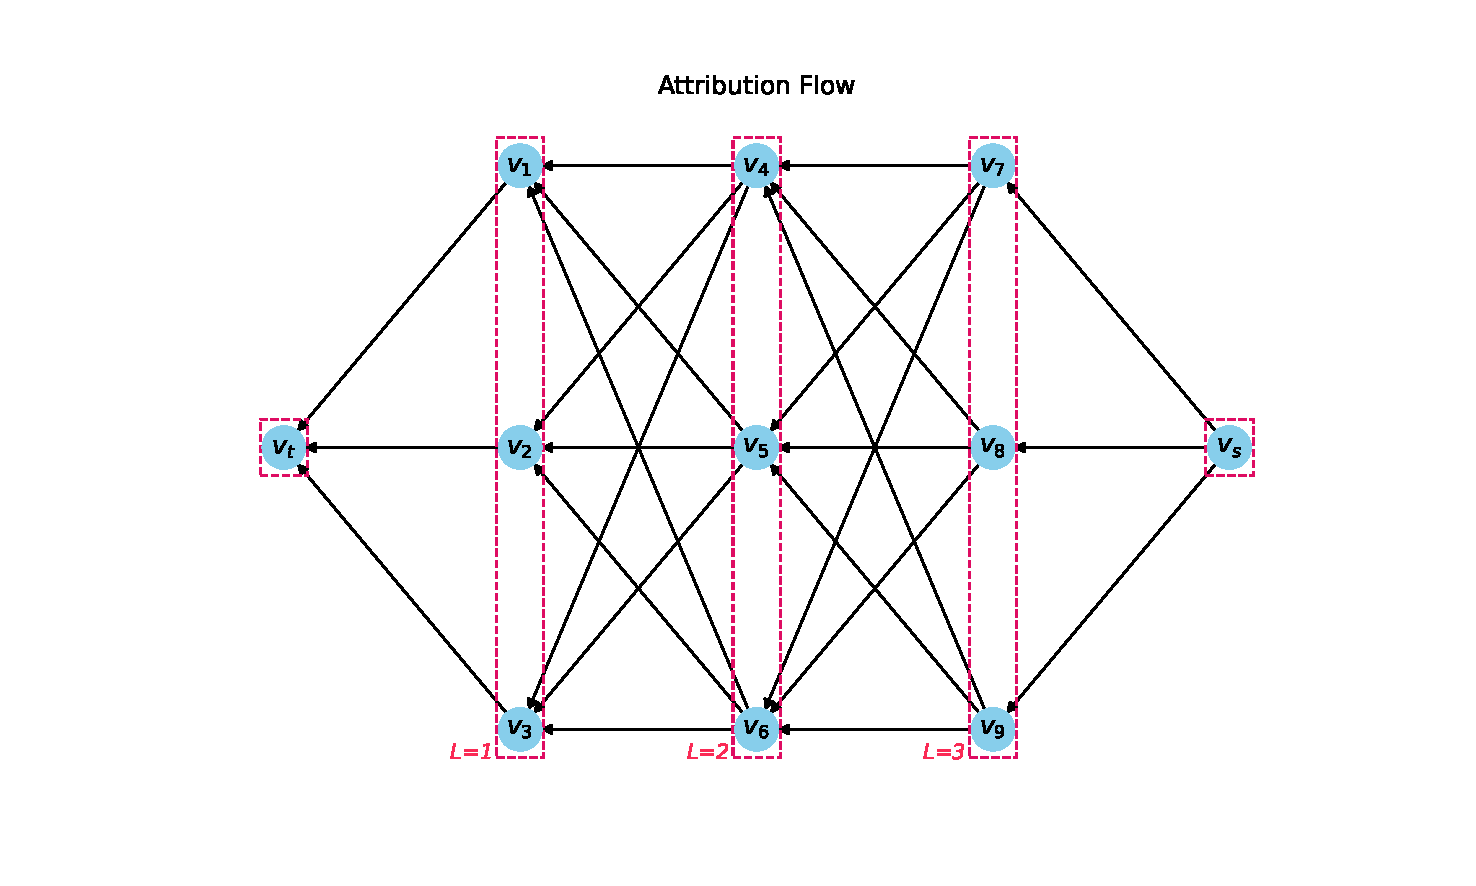
\includegraphics[width=10.5cm, height=6cm]{Figs/attribution_flow_bw.pdf}\hspace{-1.5cm}}
%		}
%	\subfloat[forward attribution flow]{
%		{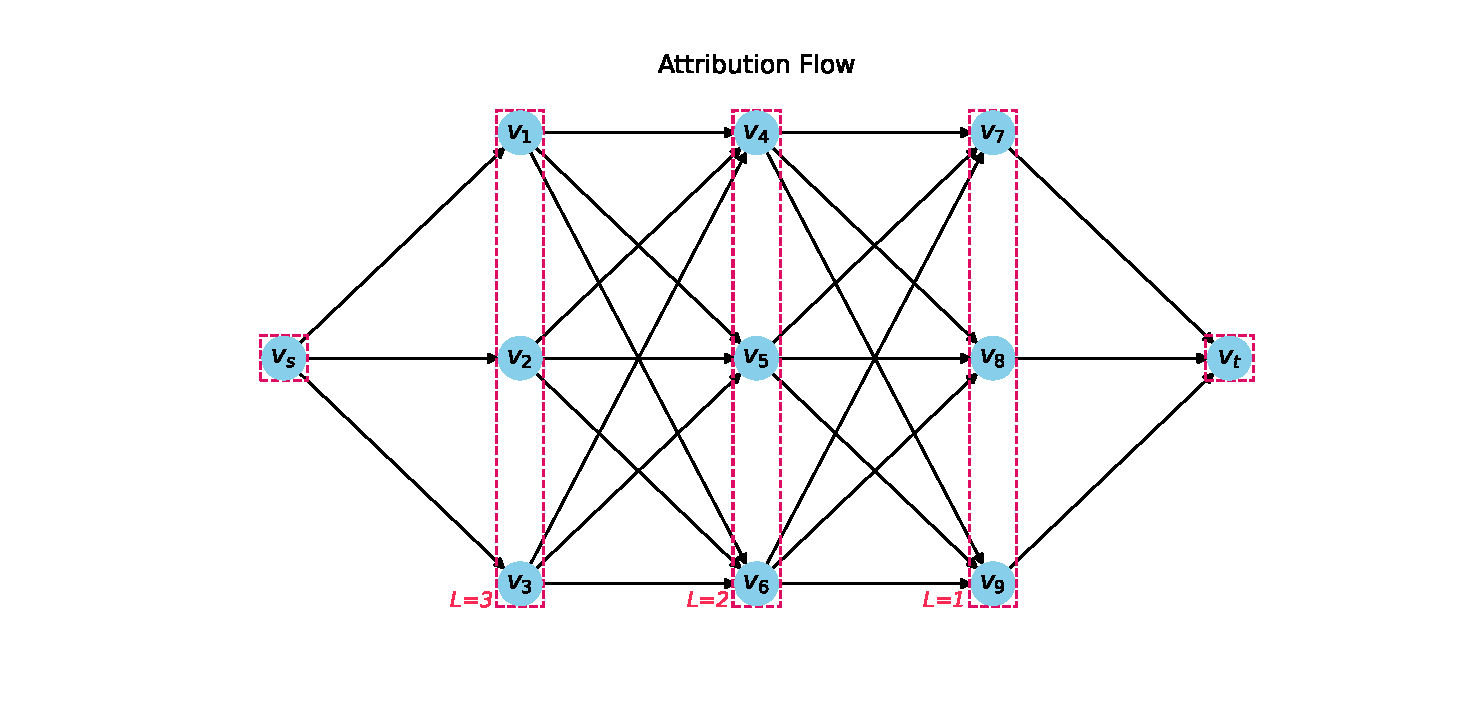
\includegraphics[width=10.5cm, height=6cm]{Figs/attribution_flow_fw.pdf} }
%		}
%%		\qquad
%%	\subfloat[label1c]{
%%		{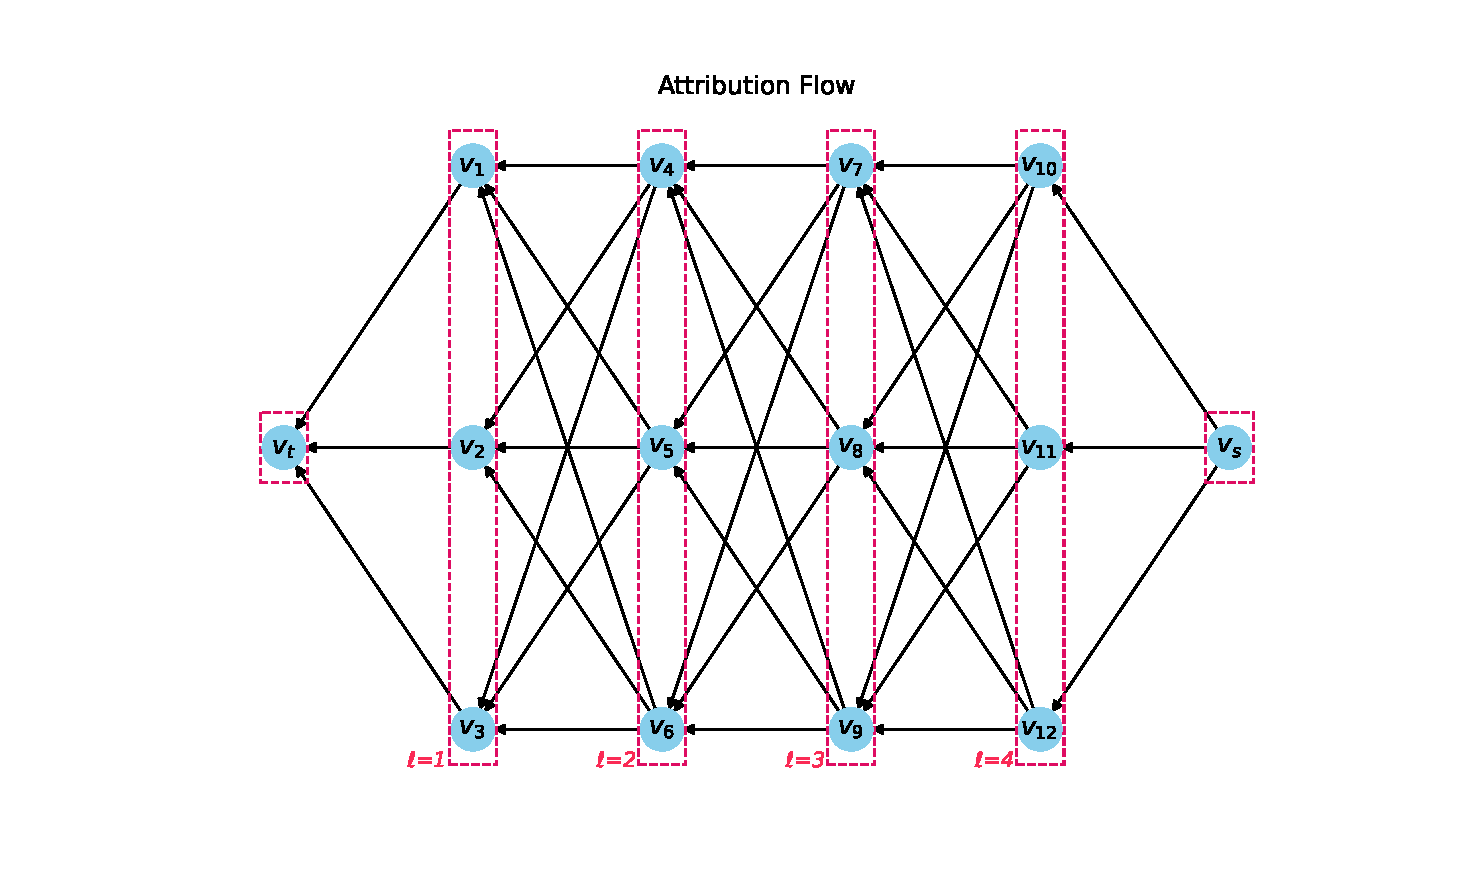
\includegraphics[width=4cm]{Figs/Attribution_flow-0.pdf}}
%%		}%
%%	\subfloat[label1d]{
%%		{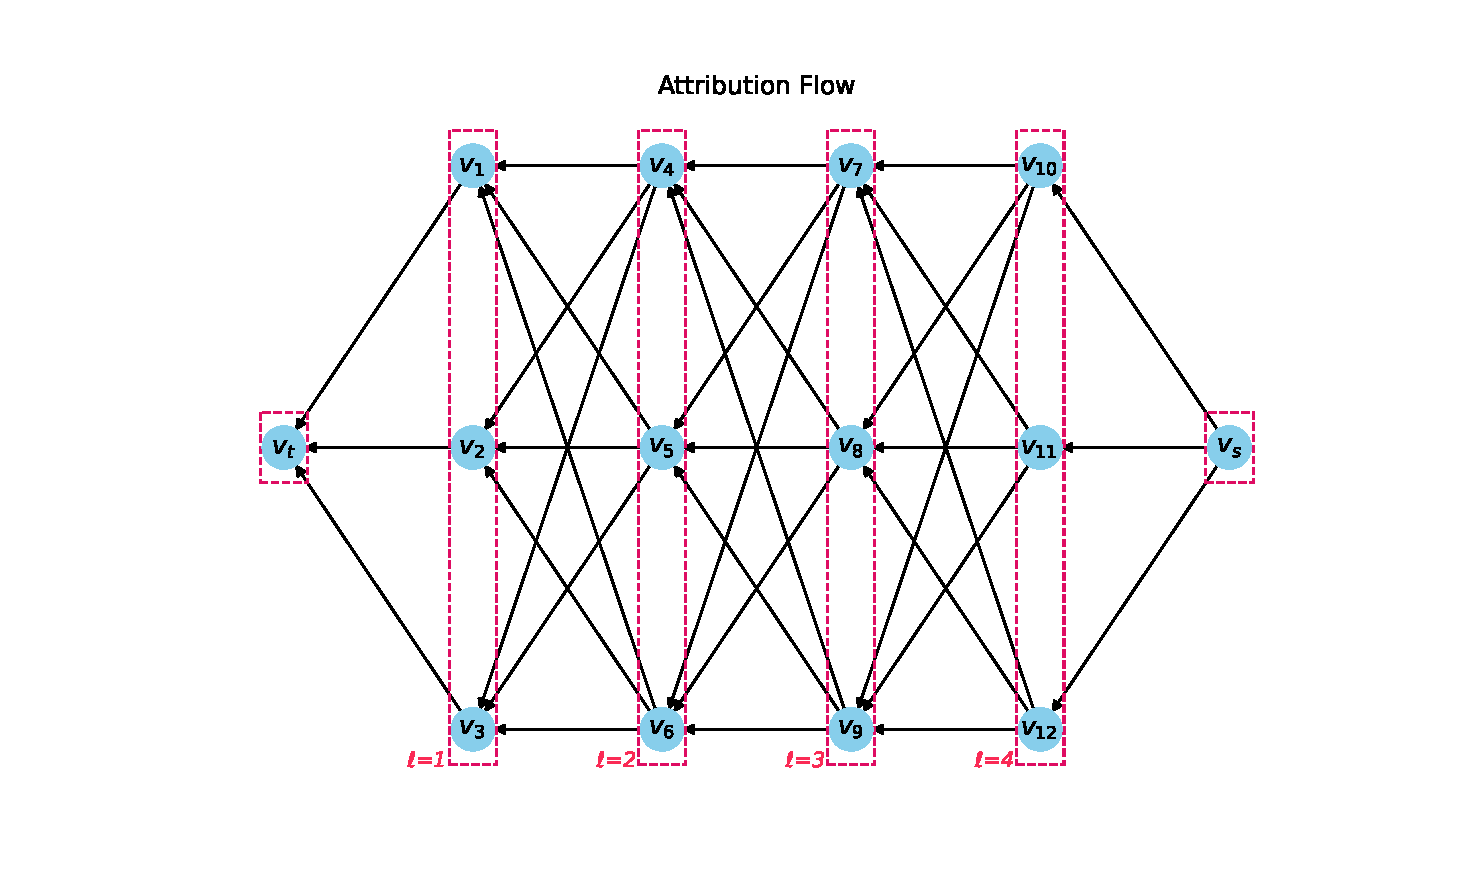
\includegraphics[width=4cm]{Figs/Attribution_flow-0.pdf}}
%%		}%
%	\caption{four side by side}
%	\label{fig:4_models}
%\end{figure} 

\begin{theorem}[Shapley Values]
	Given a directed multi-partite attribution graph $\mathcal{G}$ defined above, assume $\bm{f}^{\ast}$ be the optimal unique solution of \cref{eq:9}  or \cref{eq:10}, and $N \subseteq V$ such that all nodes in $N$ are chosen from the same partite (layer). For every  $S \subseteq N$, define the payoff function $\vartheta(S)=|\bm{f}^{\ast}(S)|$. Therefore for each node $i \in N$, $\phi_i(\vartheta)= |f_{out}(i)|$ is Shapley value.
\end{theorem}


\section{Instantiation}
Te main ingredient to construct our attribution flow is the tensor  $\bm{F} \in \mathbb{R}^{l \times t \times t}$. Here, we introduce some well known attribution flow which can be used to get the Shapley values.\citep{barkan2021, jain2020, chefer2021a, chefer2021d}

\begin{enumerate}
	\item $\textbf{Attention: } \bm{F} := \mathbb{E}_h(\bm{A})$
	\item $\textbf{Attention Grad: } \bm{F} := \mathbb{E}_h(\lfloor \nabla \hspace{-1.75pt} \bm{A} \rfloor_{\!+})$
	\item  $\textbf{Attention $\times$ Attention Grad: } \bm{F} := \mathbb{E}_h(\lfloor \bm{A} \odot \nabla \hspace{-1.75pt} \bm{A} \rfloor_{\!+})$
\end{enumerate}
In the above formulas $\lfloor x \rfloor_{\!+} = \max(x, 0)$, $\odot$ is the Hadamard product, and $\mathbb{E}_h$ is the mean across the "heads" dimension.

It is noteworthy that we can also consider any subset of tokens and get their Shapley Values, which can be done by either:
\begin{itemize}
	\item removing the corresponding columns and rows of the removed tokens from attribution flow $\bm{F}$ and create $\bm{F}^{\ast} \in \mathbb{R} ^{l \times r \times r }$  where $r$ is the cardinality of the remained tokens.
	
	\item setting the corresponding columns and rows of the removed tokens from attribution flow $\bm{F}$ to zero.
\end{itemize}
It is clear that both methods provide the same Shapley values.




%%%%%%%%%%%%%%%%%%%%%%%%%%%%%%%%%%%%%%%%%%%%%%%%%%%%%%%%%%%%%%%%%%%%%%%%%%%%%%%%%%%%%%%%%%%%%%%%%%%
\pagebreak

%\def\bibfont{\small} % set bibliography font size to small
%\setlength{\bibsep}{8 pt} % set 4 pt spacing between entries


\bibliography{iclr2024_conference}
\bibliographystyle{iclr2024_conference}

%%%%%%%%%%%%%%%%%%%%%%%%%%%%%%%%%%%%%%%%%%%%%%%%%%%%%%%%%%%%%%%%%%%%%%%%%%%%%%%%%%%%%%%%%%%%%%%%%%%
\pagebreak
\appendix
\section{Appendix}
You may include other additional sections here.

\subsection{Definitions}

\subsubsection{Multi-Commodity Maximum Flow}
The multi-commodity flow problem is an important variant of the maximum flow problem. This problem involves multiple source-sink pairs, unlike the standard maximum flow problem which only considers one source and one sink. The goal is to find multiple feasible flows, denoted by $f^1(\cdot, \cdot), \ldots, f^r(\cdot, \cdot)$, where each $f^k(\cdot, \cdot)$ represents a feasible flow from the source $s_k$ to the sink $t_k$. The objective is to ensure that all capacity constraints are satisfied, which are represented by the equation:

\begin{equation*}
	\sum_{k=1}^r f^k(i, j) \leq u(i, j) \quad \forall(i, j) \in E
\end{equation*}

Such a flow is known as a "multi-commodity" flow. A multi-commodity maximum flow problem is to maximize the function $\sum_{k=1}^r \sum_{v:(v, s_k)} f^k_{s_k v}$.


To solve the problem of multi-commodity maximum flow, we can simplify it by transforming it into a standard maximum flow problem. This can be achieved by introducing two new nodes - a "super-source" node $s$ and a "super-sink" node $t$. The "super-source" node $s$ should be connected to all the original sources $s_i$ through edges of finite capacities, while the "super-sink" node $t$ should be connected to all the original sinks $t_i$ with edges of finite capacities:

\begin{itemize}
	\item Each outgoing edge from the "super-source" node $s$ to each source
	node $s_i$ gets assigned a capacity that is equal to the total capacity of the
	outgoing edges from the source node $s_i$.
	
	\item Each incoming edge from an original "super-sink" node $t$ to each sink
	node $t_i$ gets assigned a capacity that is equal to the total capacity of the
	incoming edge to the sink node $t_i$.
\end{itemize}

It is easy to see that the maximum flow from $s$ to $t$ is equivalent to the maximum sum of flows in a feasible multi-commodity flow in the original network.


\subsubsection{Minimum Cost Circulation Problem}

The formulation of minimum-cost circulation problem can be written as the following linear programming (LP) problem:

\begin{equation}
	\underset{\substack{\bm{B}^{\top} \bm{f}=\bm{0} \\ l_e \leq f_e \leq u_e \forall e \in E}}{\min } \hspace{-4pt} \bm{c}^{\top} \bm{f} \quad  \text{i.e.}	\quad 
	\underset{\substack{\bm{B}^{\top} \bm{f}=\bm{0} \\ \bm{l} \leq \bm{f} \leq \bm{u} }}{\arg \min } \hspace{4pt} \bm{c}^{\top} \bm{f}	
	\label{eq:5}
\end{equation}


It is easy to show that it satisfies strong duality with dual problem:
\begin{equation}
	\max _{\substack{\bm{B} \bm{y}+\bm{s}_{l}-\bm{s}_{u}=\bm{c}\\ \bm{s}_{l}, \bm{s}_{u} \in \mathbb{R}_{\geq 0}^E}} \hspace{-4pt} -\bm{s}_u^{\top} \bm{u}+\bm{s}_l^{\top} \bm{l}
	\label{eq:6}
\end{equation}

where the Lagrangian (\(\mathcal{L}\)) is defined as:
\[
\begin{aligned}
	\mathcal{L}(\bm{f}, \bm{y}, \bm{s}_{u}, \bm{s}_{l}) &= \bm{c}^{\top} \bm{f} + \bm{y}^{\top}(\bm{B}^{\top} \bm{f}) + \bm{s}_u^{\top}(\bm{u} - \bm{f}) + \bm{s}_l^{\top}(\bm{f} - \bm{l})
\end{aligned}
\]

Since our primal LP problem is convex, the  KKT conditions provide both necessary an sufficient conditions to find optimal primal and dual variables for the minimum cost circulation problem as follows:
\begin{enumerate}
	\item \textbf{Stationarity}:
	\[
	\begin{aligned}
		\nabla \mathcal{L}(\bm{f}, \bm{y}, \bm{s}_{u}, \bm{s}_{l}) &= \bm{c} - \bm{B}\bm{y} + \bm{s}_{u} - \bm{s}_{l} = \bm{0}
	\end{aligned}
	\]
	
	\item \textbf{Complementary Slackness}:
	\[
	\begin{aligned}
		& \bm{s}_u^{\top}(\bm{u} - \bm{f}) = \bm{0}:  s_e^+ \cdot (u_e - f_e)= 0, \quad \forall e \in E \quad (\text{for upper-bound capacity constraints}) \\
		& \bm{s}_l^{\top}(\bm{f} - \bm{l}) = \bm{0}:  s_e^- \cdot (f_e - l_e)= 0, \quad \forall e \in E \quad(\text{for lower-bound capacity constraints})
	\end{aligned}
	\]
	
	\item \textbf{Primal Feasibility}:
	\[
	\begin{aligned}
		\bm{B}^{\top}\bm{f} &= \bm{0} \quad (\text{flow conservation constraint}) \\
		\bm{l} \leq \bm{f} \leq \bm{u}: \hspace{8pt} l_e \leq f_e &\leq u_e, \quad \forall e \in E \quad (\text{capacity constraints})
	\end{aligned}
	\]
	
	\item \textbf{Dual Feasibility}:
	\[
	\begin{aligned}
		\bm{s}_{u}, \bm{s}_{l} &\geq \bm{0} \quad (\text{non-negativity of slack variables})
	\end{aligned}
	\]
\end{enumerate}


Here, \(\bm{y}\) represents the dual variables corresponding to the equality constraint (\(\bm{B}^{\top}\bm{f} = \bm{0}\)), and \(\bm{s}_{u}\) and \(\bm{s}_{l}\) represent the dual variables corresponding to the upper and lower inequality constraints (\(l_e \leq f_e \leq u_e\)), respectively.


\subsubsection{Shapley Values}

The Shapley value, introduced by \cite{shapley1952}, concerns the cooperative game in the coalitional form $(N, \vartheta)$, where $N$ is a set of $n$ players and $\vartheta: 2^N \rightarrow \mathbb{R}$ with $\vartheta(\emptyset)=0$ is the characteristic function. In the game, the marginal contribution of the player $i$ to any coalition $S$ with $i \notin S$ is considered as $\vartheta(S \cup i)-\vartheta(S)$. These Shapley values are the only constructs that jointly satisfy the Efficiency, Symmetric, Null Player and Additivity axioms:

\begin{itemize}
	
	\item \textbf{Efficiency:} The Shapley values must add up to the total value of the game, which means $\sum_{i \in N} \phi_i(\vartheta) = \vartheta(N)$
	\item \textbf{Symmetry:} If two players are equal in their contributions to any coalition, they should receive the same Shapley value. Mathematically, if \(\vartheta(S \cup \{i\}) = \vartheta(S \cup \{j\})\) for all \(S \subseteq N \setminus \{i, j\}\), then \(\phi_i(\vartheta) = \phi_j(\vartheta)\).
	\item \textbf{Null Player:} If a player has no impact on any coalition, their Shapley value should be zero. Mathematically, if \(\vartheta(S \cup \{i\}) = \vartheta(S)\) for all \(S \subseteq N \setminus \{i\}\), then \(\phi_i(\vartheta) = 0\).
	\item \textbf{Linearity:} If two games are combined into a larger game, the Shapley value of a player in the combined game is the sum of their Shapley values in the individual games.
	
\end{itemize}

 By considering these axioms, the attribution of a player $i$ is uniquely given by:

\begin{equation*}
	\phi_j(\vartheta)=\mathlarger{\sum\limits_{S \subseteq N \backslash\{j\}}} \frac{|S| !(n-|S|-1) !}{n !}(\vartheta(S \cup\{j\})-\vartheta(S))
\end{equation*}

\section{Proofs}

\begin{proof}
	Since the optimal flow $bm{f}^{\ast}$ is only calculated once, with the entire graph, and not for each possible subgraph, and the players are all disjoint and have no connections in $S$, blocking the flow through one player does not affect the outflow of any of the other players (tokens).
	Therefore, it is easy o check that for every $S \subseteq N$ that $i \notin S$  we have  $|f_{out}(i)| = v(S \cup\{i\})-v(S)$. Employing the defintion of the Shapley values in \cref{eq:4}, we will have:
	
	\begin{equation*}
		\begin{aligned}
			\phi_i(\vartheta) & =\mathlarger{\sum\limits_{S \subseteq N \backslash\{i\}}} \frac{|S| !(n-|S|-1) !}{n !}(\vartheta(S \cup\{i\})-\vartheta(S)) \\
			& =\mathlarger{\sum\limits_{S \subseteq N \backslash\{i\}}} \frac{|S| !(n-|S|-1) !}{n !}(|f_{out}(i)|) \\
			& = |f_{out}(i)|\mathlarger{\sum\limits_{S \subseteq N \backslash\{i\}}} \frac{|S| !(n-|S|-1) !}{n!} \\
			& = |f_{out}(i)|
		\end{aligned}
	\end{equation*}
\end{proof}

\end{document}
